% Options for packages loaded elsewhere
\newgeometry{
    margin=0.75cm,
    noheadfoot, nomarginpar,
    footskip=1.25em,
}
\begin{landscape}
\section{Supplementary}

\begin{table}[H]
\centering
\caption{Spatial model summaries for Est  describing effective and nominal dimensions, their ratio, and parameter type across all traits}
\centering
\resizebox{\linewidth}{!}{
\begin{tabular}[t]{lllllllllllll}
\toprule
\multicolumn{1}{c}{} & \multicolumn{4}{c}{TY} & \multicolumn{4}{c}{TN} & \multicolumn{4}{c}{TV} \\
\cmidrule(l{3pt}r{3pt}){2-5} \cmidrule(l{3pt}r{3pt}){6-9} \cmidrule(l{3pt}r{3pt}){10-13}
    & \makecell{Effective\\Dimension} & \makecell{Nominal\\Dimension} & Ratio & Type\textsuperscript{a} & \makecell{Effective\\Dimension} & \makecell{Nominal\\Dimension} & Ratio & Type\textsuperscript{a} & \makecell{Effective\\Dimension} & \makecell{Nominal\\Dimension} & Ratio & Type\textsuperscript{a}\\
\midrule
Intercept & 1.0 & 1 & 1.00 & F & 1.0 & 1 & 1.00 & F & 1.0 & 1 & 1.00 & F\\
Control & 1.0 & 1 & 1.00 & F & 1.0 & 1 & 1.00 & F & 1.0 & 1 & 1.00 & F\\
Genotype & 505.5 & 604 & 0.84 & R & 483.0 & 604 & 0.80 & R & 539.6 & 604 & 0.89 & R\\
R-Row & 12.2 & 18 & 0.68 & R & 12.2 & 18 & 0.68 & R & 8.5 & 18 & 0.47 & R\\
R-Column & 0.0 & 63 & 0.00 & R & 0.0 & 63 & 0.00 & R & 0.0 & 63 & 0.00 & R\\
\addlinespace
Column & 1.0 & 1 & 1.00 & S & 1.0 & 1 & 1.00 & S & 1.0 & 1 & 1.00 & S\\
Row & 1.0 & 1 & 1.00 & S & 1.0 & 1 & 1.00 & S & 1.0 & 1 & 1.00 & S\\
Column:Row & 1.0 & 1 & 1.00 & S & 1.0 & 1 & 1.00 & S & 1.0 & 1 & 1.00 & S\\
f(Column) & 2.9 & 21 & 0.14 & S & 3.4 & 21 & 0.16 & S & 0.9 & 21 & 0.04 & S\\
f(Row) & 0.0 & 66 & 0.00 & S & 0.0 & 66 & 0.00 & S & 0.0 & 66 & 0.00 & S\\
\addlinespace
f(Column):Row & 3.8 & 21 & 0.18 & S & 0.0 & 21 & 0.00 & S & 3.0 & 21 & 0.14 & S\\
Column:f(Row) & 0.7 & 66 & 0.01 & S & 0.6 & 66 & 0.01 & S & 0.0 & 66 & 0.00 & S\\
f(Column):f(Row) & 16.5 & 1386 & 0.01 & S & 11.7 & 1386 & 0.01 & S & 2.9 & 1386 & 0.00 & S\\
 &  &  &  &  &  &  &  &  &  &  &  & \\
Total & 546.7 & 2250 & 0.24 &  & 515.9 & 2250 & 0.23 &  & 559.8 & 2250 & 0.25 & \\
\addlinespace
Residual & 635.3 &  &  &  & 666.1 &  &  &  & 622.2 &  &  & \\
\bottomrule
\multicolumn{13}{l}{\rule{0pt}{1em}\textsuperscript{a} F = Fixed, R = Random, S = Semi-parametric}\\
\end{tabular}}
\end{table}

\end{landscape}
\restoregeometry

\begin{landscape}

\begin{table}
\centering
\caption{Spatial model summaries for Heelsum describing effective and nominal dimensions, their ratio, and parameter type across all traits}
\centering
\resizebox{\ifdim\width>\linewidth\linewidth\else\width\fi}{!}{
\begin{tabular}[t]{lllllllllllll}
\toprule
\multicolumn{1}{c}{} & \multicolumn{4}{c}{TY} & \multicolumn{4}{c}{TN} & \multicolumn{4}{c}{TV} \\
\cmidrule(l{3pt}r{3pt}){2-5} \cmidrule(l{3pt}r{3pt}){6-9} \cmidrule(l{3pt}r{3pt}){10-13}
  & Effective Dimension & Nominal Dimension & Ratio & Type\textsuperscript{a} & Effective Dimension & Nominal Dimension & Ratio & Type\textsuperscript{a} & Effective Dimension & Nominal Dimension & Ratio & Type\textsuperscript{a}\\
\midrule
Intercept & 1.0 & 1 & 1.00 & F & 1.0 & 1 & 1.00 & F & 1.0 & 1 & 1.00 & F\\
Control & 1.0 & 1 & 1.00 & F & 1.0 & 1 & 1.00 & F & 1.0 & 1 & 1.00 & F\\
Genotype & 634.0 & 718 & 0.88 & R & 585.6 & 718 & 0.82 & R & 643.0 & 718 & 0.90 & R\\
R-Row & 0.0 & 18 & 0.00 & R & 0.0 & 18 & 0.00 & R & 0.0 & 18 & 0.00 & R\\
R-Column & 37.3 & 83 & 0.45 & R & 39.7 & 83 & 0.48 & R & 45.3 & 83 & 0.55 & R\\
\addlinespace
Column & 1.0 & 1 & 1.00 & S & 1.0 & 1 & 1.00 & S & 1.0 & 1 & 1.00 & S\\
Row & 1.0 & 1 & 1.00 & S & 1.0 & 1 & 1.00 & S & 1.0 & 1 & 1.00 & S\\
Column:Row & 1.0 & 1 & 1.00 & S & 1.0 & 1 & 1.00 & S & 1.0 & 1 & 1.00 & S\\
f(Column) & 4.5 & 21 & 0.21 & S & 3.2 & 21 & 0.15 & S & 2.2 & 21 & 0.10 & S\\
f(Row) & 0.0 & 86 & 0.00 & S & 0.4 & 86 & 0.01 & S & 0.9 & 86 & 0.01 & S\\
\addlinespace
f(Column):Row & 0.0 & 21 & 0.00 & S & 0.2 & 21 & 0.01 & S & 0.0 & 21 & 0.00 & S\\
Column:f(Row) & 0.0 & 86 & 0.00 & S & 0.3 & 86 & 0.00 & S & 0.0 & 86 & 0.00 & S\\
f(Column):f(Row) & 18.3 & 1806 & 0.01 & S & 13.3 & 1806 & 0.01 & S & 6.4 & 1806 & 0.00 & S\\
 &  &  &  &  &  &  &  &  &  &  &  & \\
Total & 699.2 & 2844 & 0.25 &  & 647.6 & 2844 & 0.23 &  & 702.8 & 2844 & 0.25 & \\
\addlinespace
Residual & 771.8 &  &  &  & 823.4 &  &  &  & 731.2 &  &  & \\
\bottomrule
\multicolumn{13}{l}{\rule{0pt}{1em}\textsuperscript{a} F = Fixed, R = Random, S = Semi-parametric}\\
\end{tabular}}
\end{table}

\end{landscape}

\begin{table}
\centering
\caption{Variance components from hybrid model with standard errors included in parantheticals for total tuber number (TN), average tuber volume (TV), and total tuber yield (TY). Covariances between traits excluded here for brevity.}
\centering
\begin{tabular}[t]{llll}
\toprule
Component & TN & TV & TY\\
\midrule
$\sigma^2_G$ & 1432.98 (131.33) & 27.29 (2.04) & 25.60 (2.42)\\
$\sigma^2_{GE}$ & 589.55 (73.30) & 5.27 (0.60) & 15.06 (1.41)\\
$\sigma^2_\varepsilon$ & 923.07 (43.72) & 6.66 (0.32) & 11.84 (0.56)\\
\bottomrule
\end{tabular}
\end{table}

\begin{figure}[H]

{\centering \pandocbounded{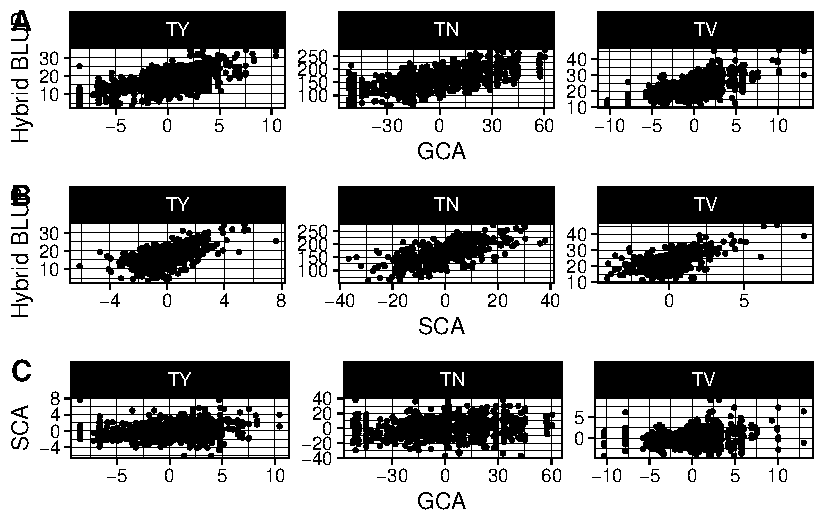
\includegraphics[keepaspectratio]{figs_02/bv-sca-performance-1.pdf}}

}

\caption{Scatterplots for each tuber trait with (A) hybrid BLUP's
plotted with GCA's, (B) SCA's, and (C) GCA's on SCA's}

\end{figure}%

\begin{table}
\centering
\caption{Ratio between the sample quantiles of GCA and SCA effects for total yield (TY), tuber number (TN), and average tuber volume (TV). Included are the 0, 10th, 25th, 40th, 60th, 75th, 90th and 100th percentiles along with an average ratio of quantiles in $\overline{q}$.}
\centering
\begin{tabular}[t]{lrrrrrrrrr}
\toprule
Trait & 0\% & 10\% & 25\% & 40\% & 60\% & 75\% & 90\% & 100\% & $\overline{q}$\\
\midrule
TN & 1.4 & 2.0 & 2.4 & 2.4 & 2.5 & 2.1 & 2.2 & 1.6 & 2.1\\
TV & 2.5 & 2.0 & 1.7 & 1.6 & 1.8 & 2.1 & 1.7 & 1.4 & 1.9\\
TY & 1.4 & 2.4 & 2.0 & 2.4 & 2.3 & 2.5 & 2.0 & 1.4 & 2.0\\
\bottomrule
\end{tabular}
\end{table}
